
\section{Evaluation}
\label{sec:Evaluation}
We present our evaluation in two parts. First, we evaluate our programmable SumCheck unit as a standalone unit in \autoref{sec:standalone_sumcheck}. We use polynomial gates seen in prior works \cite{verifiable_asics, spartan} as well as gates used for elliptic curve addition in the Halo2 \cite{halo2} library. We then evaluate it as part of a broader HyperPlonk accelerator, zkPHIRE, in \autoref{sec:zkphire_eval}.


\begin{table}[t]
    \caption{List of polynomial constraints.}
    \label{tab:polynomials}
    \centering
    \begin{tabular}{|c|c|c|}
        \hline
        \textbf{ID} & \textbf{Name} & \textbf{Polynomial} \\
        \hline
        0 & Verifiable ASICs \cite{verifiable_asics} & $q_{\text{add}}\cdot(a + b) + q_{\text{mul}}\cdot(a \cdot b)$ \\
        \hline
        1 & Spartan 1 \cite{spartan} & $(A \cdot B - C) \cdot f_\tau$ \\
        \hline
        2 & Spartan 2 \cite{spartan} & $(\text{Sum}_{ABC}) \cdot Z$ \\
        \hline
        \multicolumn{3}{|c|}{\textbf{Halo2 Constraints \cite{halo2}}} \\
        \hline
        3 & Nonzero Point Check & $q_\text{point}^\text{non-id} \cdot (y^2 - x^3 - 5)$ \\
        \hline
        4 & $x$-gated Curve Check & $(q_\text{point} \cdot x) \cdot (y^2 - x^3 - 5)$ \\
        \hline
        5 & $y$-gated Curve Check & $(q_\text{point} \cdot y) \cdot (y^2 - x^3 - 5)$ \\
        \hline
        6 & Incomplete Addition 1 & \makecell[c]{$q_\text{add-incomplete} \cdot ((x_r + x_q + x_p) $ \\  $\cdot(x_p - x_q)^2 - (y_p - y_q)^2)$} \\
        \hline
        7 & Incomplete Addition 2 & \makecell[c]{$q_\text{add-incomplete} \cdot  (y_r + y_q)(x_p - x_q)$ \\ $- (y_p - y_q)(x_q - x_r)$} \\
        \hline
        8 & Complete Addition 1 & \makecell[c]{$q_\text{add} \cdot (x_q - x_p)((x_q - x_p)\lambda$ \\ $- (y_q - y_p))$} \\
        \hline
        9 & Complete Addition 2 & \makecell[c]{$q_\text{add} \cdot (1 - (x_q - x_p)\alpha)$ \\ $(2y_p\lambda - 3x_p^2)$} \\
        \hline
        10 & Complete Addition 3 & \makecell[c]{$q_\text{add} \cdot x_p x_q (x_q - x_p)$ \\ $(\lambda^2 - x_p - x_q - x_r)$} \\
        \hline
        11 & Complete Addition 4 & \makecell[c]{$q_\text{add} \cdot x_p x_q (x_q - x_p)$ \\ $(\lambda(x_p - x_r) - y_p - y_r)$} \\
        \hline
        12 & Complete Addition 5 & \makecell[c]{$q_\text{add} \cdot x_p x_q (y_q + y_p)$ \\ $(\lambda^2 - x_p - x_q - x_r)$} \\
        \hline
        13 & Complete Addition 6 & \makecell[c]{$q_\text{add} \cdot x_p x_q (y_q + y_p)$ \\ $(\lambda(x_p - x_r) - y_p - y_r)$} \\
        \hline
        14 & Complete Addition 7 & $q_\text{add} \cdot (1 - x_p \cdot \beta)(x_r - x_q)$ \\
        \hline
        15 & Complete Addition 8 & $q_\text{add} \cdot (1 - x_p \cdot \beta)(y_r - y_q)$ \\
        \hline
        16 & Complete Addition 9 & $q_\text{add} \cdot (1 - x_q \cdot \gamma)(x_r - x_p)$ \\
        \hline
        17 & Complete Addition 10 & $q_\text{add} \cdot (1 - x_q \cdot \gamma)(y_r - y_p)$ \\
        \hline
        18 & Complete Addition 11 & \makecell[c]{$q_\text{add} \cdot (1 - (x_q - x_p)\alpha$ \\ $- (y_q + y_p)\delta)x_r$} \\
        \hline
        19 & Complete Addition 12 & \makecell[c]{$q_\text{add} \cdot (1 - (x_q - x_p)\alpha$ \\ $- (y_q + y_p)\delta)y_r$} \\
        \hline
        \multicolumn{3}{|c|}{\textbf{HyperPlonk (HP) Polynomials \cite{hyperplonk} }} \\
        \hline
        20 & Vanilla ZeroCheck & \makecell[c]{$(q_Lw_1 + q_Rw_2 - q_Ow_3$ \\$+ q_Mw_1w_2 +q_C)f_r$} \\
        \hline
        21 & \makecell[c]{Vanilla PermCheck \\ ($\alpha$ is a scalar)} & \makecell[c]{
        $(\pi - p_1p_2 + \alpha(\phi D_1D_2D_3$ \\ $ - N_1N_2N_3)) f_r$} \\
        \hline
        22 & Jellyfish ZeroCheck & \makecell[c]{$(q_1 w_1 + q_2 w_2 + q_3 w_3 + q_4 w_4 $ \\ $ 
      + q_{M_1} w_1 w_2 + q_{M_2} w_3 w_4 $ \\ $+ q_{H_1} w_1^5 + q_{H_2} w_2^5 + q_{H_3} w_3^5$ \\  $+ q_{H_4} w_4^5 - q_O w_5 $\\$+ q_{ecc} w_1 w_2 w_3 w_4 + q_C) f_r$} \\
        \hline
        23 & \makecell[c]{Jellyfish PermCheck \\ ($\alpha$ is a scalar)}  & \makecell[c]{
        $(\pi - p_1p_2 + \alpha(\phi D_1D_2D_3 \cdot $ \\ $D_4D_5 - N_1N_2N_3N_4N_5)) f_r$} \\
        \hline
        24 & OpenCheck & \makecell[c]{$
        y_1f_{r_1} + y_2f_{r_2} +y_3f_{r_3} $ \\ $y_4f_{r_4} + y_5f_{r_5} +y_6f_{r_6} $} \\
        \hline
    \end{tabular}
\end{table}


\begin{figure}[t!]
    \centering
    \hspace*{-5mm} % shift left
    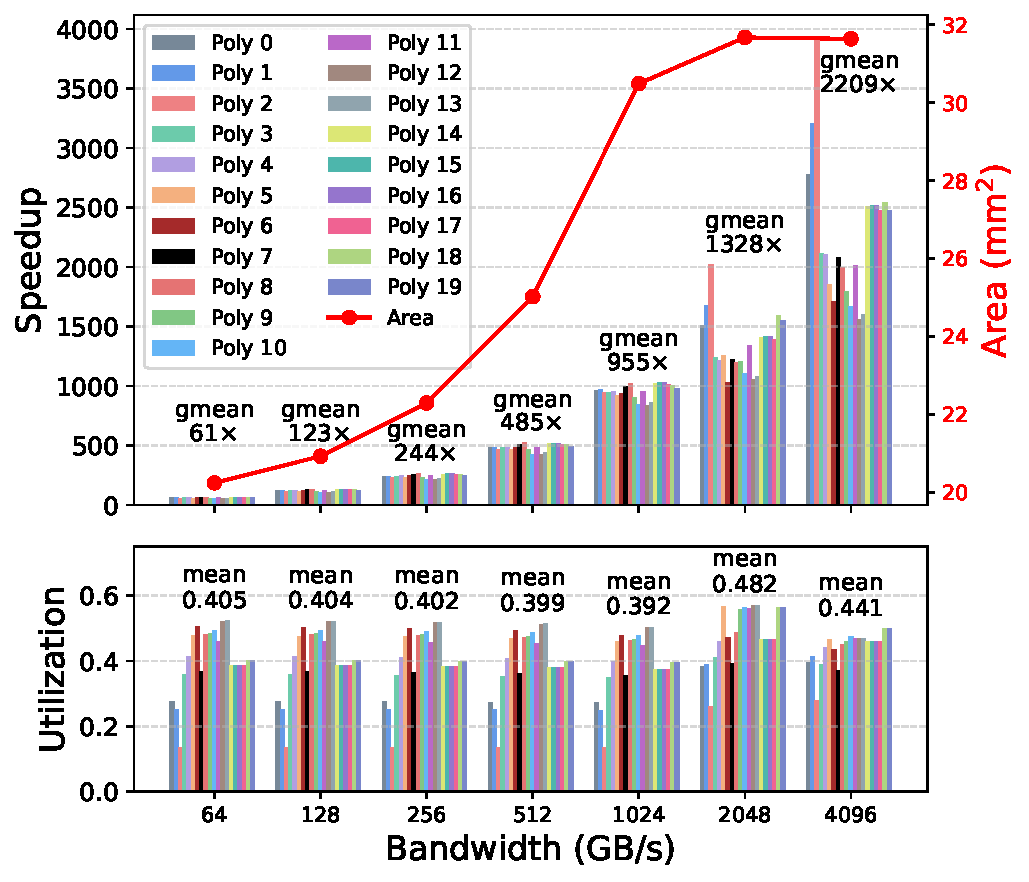
\includegraphics[width=1.08\columnwidth]{speedups_and_utilizations_combined_util_and_perf.pdf}
    \caption{Speedups over 4-threaded CPU implementations of SumChecks on the polynomials in \autoref{tab:polynomials}. We pick a different optimal design across each bandwidth technology. Utilization across the design points is also shown.}
    \label{fig:cpu_speedup_and_util}
\end{figure}

\subsection{Programmable SumCheck}
\label{sec:standalone_sumcheck}

\subsubsection{Speedup over various gate types}
\label{sec:speedup_and_util}
\autoref{tab:polynomials} enumerates the polynomials we use in our evaluation. We first benchmark the performance of SumChecks on each polynomial by extending HyperPlonk's existing code base \cite{hyperplonk}. We then run each polynomial on our programmable SumCheck unit. In this evaluation, we seek to optimize both performance and utilization across all polynomials. We can always allocate EEs and PLs to handle the worst-case polynomial degree, however, this would lead to underutilization on low-degree polynomials. In our design space search, we specify an area and bandwidth constraint and then use the following objective function:
\begin{equation*}
    \min_{\text{design}} \; (1 - \lambda) \cdot f_{\text{slowdown}}(s_{d,i}) + \lambda \cdot (1 - f_{\text{util}}(u_{d,i}))
\end{equation*}
Here, $s_{d,i}$ refers to the slowdown of the $i^{th}$ polynomial for a given design $d$, relative to the fastest runtime for that polynomial in the area-constrained design space. Similarly, $u_{d,i}$ reflects the utilization for design $d$ on polynomial $i$. $f_\text{slowdown}$ and $f_\text{util}$ are aggregation functions; we employ geomean for slowdown and arithmetic mean for utilization. $\lambda$ controls the trade-off between the minimizing slowdown and maximizing utilization. For this analysis, we focus on utilization, using $\lambda = 0.8$. We compare the runtime against the CPU running each polynomial's SumCheck on 4 threads, for which we estimate the total core area to be 37 mm$^2$ in 7nm \cite{cpu_amd1, cpu_amd2, cpu_amd3} and use that as our area constraint (after scaling from 22nm). Across various bandwidths, we find the optimal design point and report speedups and utilizations in Figure \ref{fig:cpu_speedup_and_util}. For most designs, 2 EEs and 5 PLs is optimal.

We observe $\sim$ 50\% utilization across benchmarks at each bandwidth, due to three main factors: (1) MLE Update units are inactive during the first round of SumCheck, which accounts for about half of total runtime; (2) lower-degree polynomials require fewer product lanes; and (3) repeating MLEs (e.g., $q_{add}$) reduce demand on the update modular multipliers since they are reused across terms.
Consequently, when optimizing for utilization, we observe a tendency to limit the number of EEs. Further parallelism and potentially higher utilization can be achieved by mapping multiple terms to EEs when possible, but it would introduce additional complexity in interconnect and increase bandwidth demand. These trade-offs can be explored further in future work.
In contrast, product lane modular multipliers are usually fully utilized, provided the polynomial degree and memory bandwidth are high enough.
Despite moderate utilization, we get significant speedups over CPU baselines, approaching $1000\times$ at 1 TB/s of bandwidth. 

Our SumCheck unit was benchmarked on a ``training set" of mostly lower-degree polynomials, which comprise most ZKP protocols today. However, we found that higher-degree (e.g., Jellyfish polynomials) achieved comparable or higher utilization ($\approx 47\%$) than many lower-degree polynomials. This is because additional constituent polynomials and extension products place greater concurrent demand on EEs and product lanes, indicating that the utilization improves with greater polynomial complexity for a given hardware configuration.

\subsubsection{High-degree sweep}

\begin{figure}[t!]
    \centering
    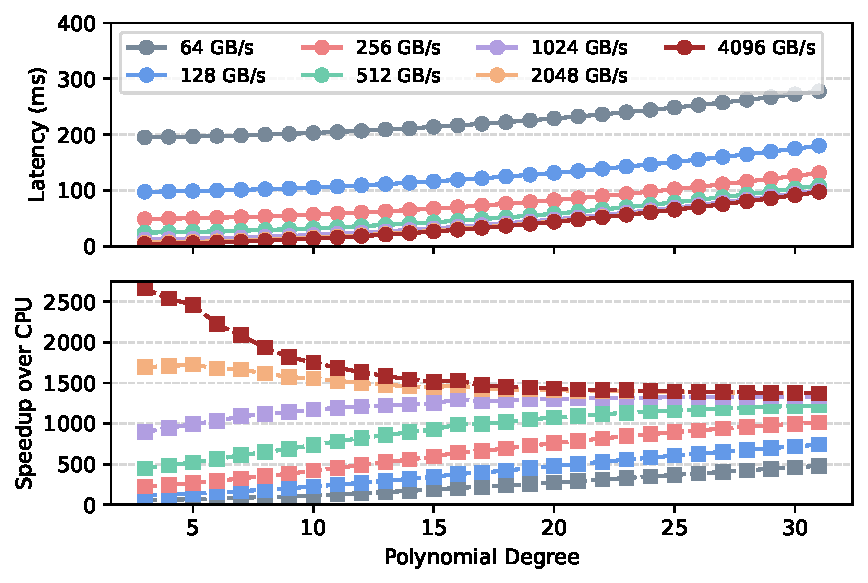
\includegraphics[width=\columnwidth]{high_degree_sweep_latencies_util_and_perf.pdf}
    \caption{Performance of a fixed SumCheck configuration on high-degree polynomials at different bandwidths. Speedup relative to CPU is also plotted.}
    \label{fig:high_degree_sweep_bw_plot}
\end{figure}

We analyze the performance scaling of SumChecks as we increase polynomial degree. We sweep polynomial degrees ($d = 2\ldots30$) for $f = q_1w_1 + q_2w_2 + q_3w_1^{d-1}w_2 + q_c$, as in HyperPlonk, and measure speedup over CPU. We use the same objective as before and pick a high-performance design under the same area constraints (\autoref{fig:high_degree_sweep_bw_plot}). Our results show that low-degree polynomials require HBM-scale bandwidths to achieve $1000\times$ speedups, while higher degree polynomials can reach similar speedups with DDR5-level bandwidths (e.g., 256 GB/s). Higher degree polynomials in this scenario exhibit more computations on the same amount of data, which is why the disparity in speedups across bandwidths is less compared to low-degree polynomials.

\begin{figure}[t!]
    \centering
    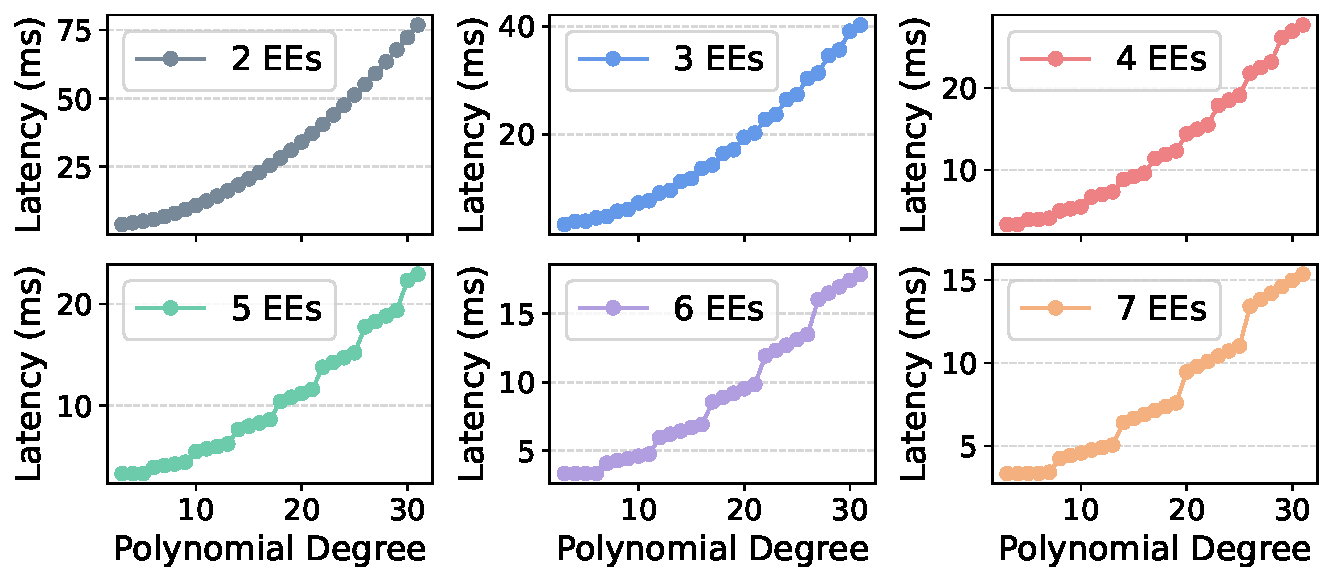
\includegraphics[width=\columnwidth]{high_degree_sweep_latencies_fixed_bw_sweep_ee.pdf}
    \caption{Scheduler-induced SumCheck behavior at fixed BW and PL settings.}
    \label{fig:ee_sweep}
\end{figure}

At fixed bandwidth, PE count, and EE-per-PE settings, increasing the number of PLs per PE improves performance roughly proportionally. Similar gains are observed when increasing EE count at fixed PLs. Interestingly, as shown in \autoref{fig:ee_sweep}, runtime increases in discrete jumps due to the graph decomposition the scheduler uses to map polynomials to EEs (see \autoref{fig:scheduler}). For example, under 6 EEs, degree-$1$–$6$ polynomials have 1 node in their schedule graph, while degree-$7$–$11$ polynomials require 2. Each added node incurs a sharp runtime jump, as it introduces additional products across all MLEs and terms. Within each node cluster, runtime grows more gradually with degree due to early exit optimizations. These trends may help optimize the SumCheck unit when the degree distribution of polynomials is known, by minimizing high-degree outliers that cause runtime spikes.


\subsubsection{Comparison with Prior ASICs}
\label{sec:asic_comp_sumcheck}
\autoref{fig:asic_speedups} details our speedups relative to a prior ASIC, zkSpeed. zkSpeed implements the SumChecks by using a custom unified core that maximizes immediate reuse. We also compare with zkSpeed+, which gives zkSpeed the benefits of pipelining MLE updates directly into the extensions and product computations (as we do in zkPHIRE). We assume the same modular multiplier area and 2 TB/s as zkSpeed. We use the same objective function from \autoref{sec:speedup_and_util} on the same training set of polynomials in \autoref{tab:polynomials} with a roughly iso-zkSpeed area constraint. We pick a 35.24 mm$^2$ design compared to zkSpeed's 30.8 mm$^2$ SumCheck and MLE Update area. Our design has 4.9 mm$^2$ of SRAM, while zkSpeed used a much larger global SRAM for storing MLEs, hence we believe this comparison is fair.

We run the same polynomials from zkSpeed's evaluation on our SumCheck unit, and find that compared to the zkSpeed+, we are only 30\% slower at iso-area and iso-bandwidth, while offering programmability to support other types of polynomials beyond those in HyperPlonk. We then use the same hardware design point for evaluation on Jellyfish polynomials. The advantage of using Jellyfish gates is that for a given application, while the polynomial complexity grows, the total gate count (i.e., workload length) decreases. We simulate three degrees of gate count reduction, $2\times, 4\times, \text{and } 8\times$.

We find that, for ZeroCheck, because the Jellyfish polynomial is more complex, the $2\times$ is not sufficient to bring speedups over the Vanilla counterpart. However, PermCheck's increase in complexity \textit{is} outweighed by a $2\times$ workload reduction. OpenCheck, which is the same between Jellyfish and Vanilla, exhibits $1.12\times, 3.54\times$ and $6.22\times$ speedup for each gate reduction over zkSpeed+. 
Combining all three SumChecks, a Jellyfish reduction by $4\times$ is sufficient to outperform Vanilla polynomials on both zkSpeed+ and zkPHIRE. These gains are observed in spite of the inherent overheads of programmability in our accelerator.

\begin{figure}[t!]
    \centering
    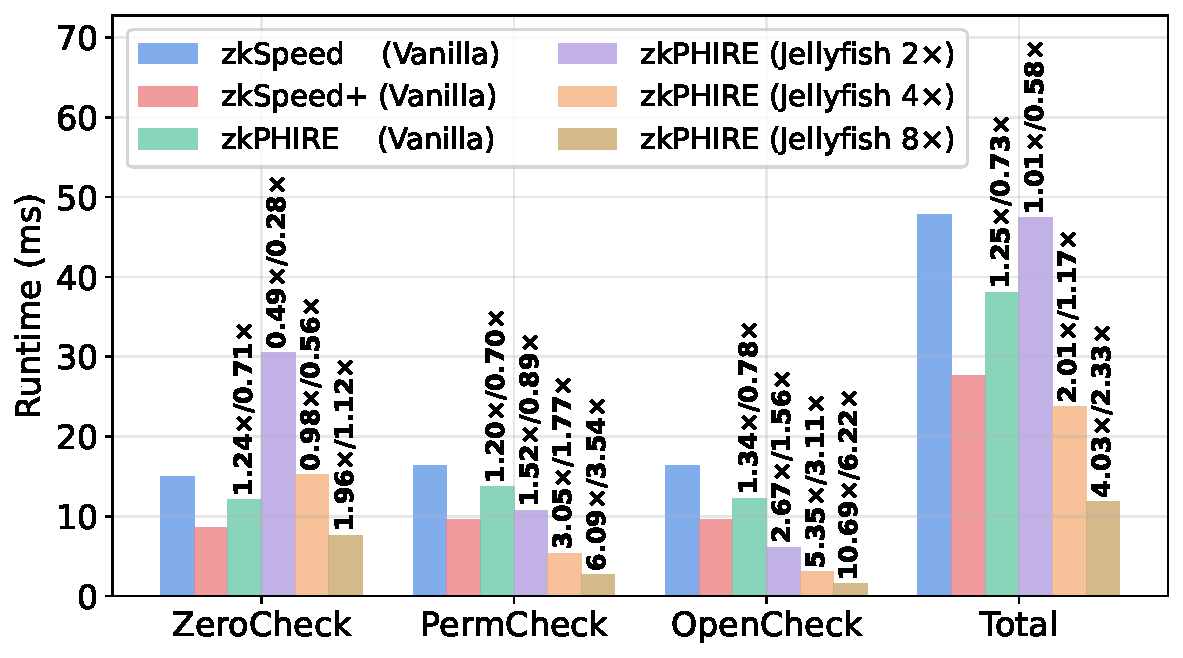
\includegraphics[width=\columnwidth]{zkspeed_only_runtime_comparison.pdf}
    \caption{Comparison with prior ASICs. Bars are annotated with speedup numbers over baseline zkSpeed / zkSpeed+. }
    \label{fig:asic_speedups}
\end{figure}

\subsubsection{Comparison with GPU}
\label{sec:gpu_comparison}
We evaluate zkPHIRE against the GPU library ICICLE~\cite{icicle} by running SumChecks from the Spartan and HyperPlonk protocols on an NVIDIA A100 GPU. 
We use the same SumCheck design from \autoref{sec:asic_comp_sumcheck}, assuming 1 TB/s of bandwidth to roughly match the A100.
Spartan is chosen due to its adoption in several recent protocols~\cite{jolt, kwan2024verifying, nova}, while HyperPlonk evaluates performance on high-degree gates.
For context, we also report CPU runtimes for these SumChecks in \autoref{tab:gpu_cpu_zkphire}.
Notably, ICICLE currently supports composite polynomials with at most eight unique constituent polynomials, preventing evaluation of polynomials 21-24 in \autoref{tab:polynomials}. We choose to evaluate the Vanilla Gate portion of polynomial 20 (excluding $f_r$).
We find that zkPHIRE accelerates these SumChecks by roughly $70\times$ over GPU, and by $600-800\times$ over CPU. 



\begin{table}[t!]
\centering
\caption{SumCheck Runtimes on CPU, GPU, and zkPHIRE for $N=24$. HyperPlonk polynomials are from \autoref{tab:polynomials}. zkPHIRE runtimes are accompanied with speedups over CPU/GPU}
\label{tab:gpu_cpu_zkphire}
\resizebox{\columnwidth}{!}{
\begin{tabular}{|c|c|c|c|c|c|}
\hline
\centering\textbf{Polynomial} & 
\centering\textbf{Number of } & 
\centering\textbf{Problem} & 
\multicolumn{3}{c|}{\textbf{Runtime (ms)}} \\ \cline{4-6}
\textbf{Type} & \textbf{SumChecks} & \textbf{Size} & \textbf{CPU} & \textbf{GPU} & \textbf{zkPHIRE} \\ \hline \hline\textbf{$(A \cdot B - C) \cdot f_\tau$} & 1  & $2^N$     & 6770  & 571  & 7.6 ($891\times$/$75\times$) \\ \hline
$(\text{Sum}_{ABC}) \cdot Z$   & 1  & $2^{N+1}$ & 5237  & 586  & 8.4  ($623\times$/$70\times$) \\ \hline
$A\cdot B \cdot C$ & 12 & $2^N$     & 60993 & 5376 &             78.9 ($773\times$/$68\times$) \\ \hline
$A\cdot B \cdot C$ & 6  & $2^{N-1}$ & 15248 & 1440 &             19.7  ($774\times$/$73\times$) \\ \hline
$A\cdot B \cdot C$ & 4  & $2^{N+1}$ & 40662 & 3460 &             52.6 ($773\times$/$66\times$) \\ \hline \hline

HP Poly. 20 \tablefootnote{$f_r$ polynomial excluded} & 1  & $2^N$ & 13354 & 1089 &  15.8 ($845\times$/$69\times$) \\ \hline
HP Poly. 21 & 1  & $2^N$ & 21625 & --  &  22.7 $(953\times)$ \\ \hline
HP Poly. 22 & 1  & $2^N$ & 74226 & --  &  69.5 $(1068\times)$ \\ \hline
HP Poly. 23 & 1  & $2^N$ & 32774 & --  &  32.2 $(1018\times)$ \\ \hline
HP Poly. 24 & 1  & $2^N$ & 17591 & --  &  21.3 $(826\times)$ \\ \hline
\end{tabular}
 }
\end{table}


\subsection{zkPHIRE}
\label{sec:zkphire_eval}

We now incorporate the programmable SumCheck unit into a larger accelerator that accelerates the HyperPlonk protocol, zkPHIRE. Here, our analysis focuses on yielding high-performance designs. In these comparisons, we assume the CPU runs with 32 threads, roughly 296 mm$^2$ in 7nm. These experiments assume fixed-prime modular multipliers, which is a common technique seen in prior work \cite{nocap, hyperplonk, libsnark}.
\begin{table}[t!]
\centering
\caption{Design Space Exploration Parameters for zkPHIRE.}
\label{tab:design_space}
\resizebox{\columnwidth}{!}{
\setlength{\tabcolsep}{2mm}{
\begin{tabular}{|c|c|c|}
\hline
\textbf{Module} & \textbf{Design Knob} & \textbf{Values}   \\ \hline \hline
\textbf{SumCheck} & PEs  & 1, 2, 4, 8, 16, 32\\ \hline
\textbf{SumCheck} & Extension Engines  & 2, 3, 4, 5, 6, 7 \\ \hline
\textbf{SumCheck} & Product Lanes  & 3, 4, 5, 6, 7, 8 \\ \hline
\textbf{SumCheck} & SRAM Bank Size  & $2^{10}-2^{15}$ \\ \hline

\textbf{MSM} & PEs                & 1, 2, 4, 8, 16, 32    \\ \hline
\textbf{MSM} & Window Size       & 7, 8, 9, 10    \\ \hline
\textbf{MSM} & Points/PE & 1K, 2K, 4K, 8K, 16K \\ \hline
\textbf{FracMLE} & PEs & 1, 2, 3, 4 \\ \hline
\textbf{---} & Bandwidth (GB/s) & 64, 128, 256, 512, 1T, 2T, 4T \\ \hline
\end{tabular}
}}
\end{table}

\begin{figure}[t!]
    \centering
    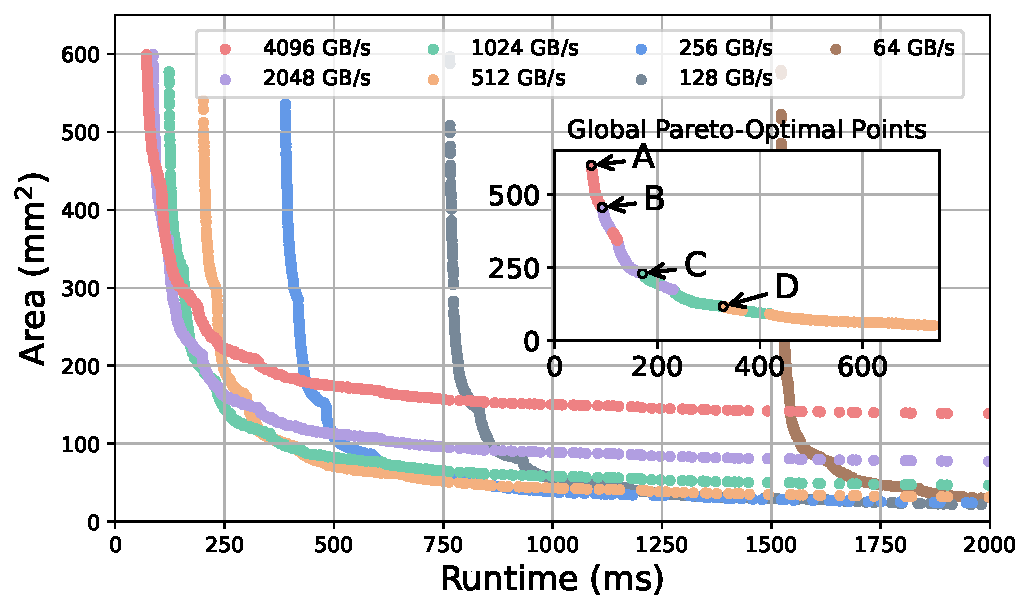
\includegraphics[width=\columnwidth]{pareto_with_global_inset_24vars_jellyfish_new.pdf}
    \caption{Pareto Frontiers for $2^{24}$ gates. We plot the individual Pareto curves for each bandwidth tier and the global Pareto frontier in the inset. We label the highest performing design for each bandwidth tier (A - D) in the inset.}
    
    \label{fig:pareto_plot}
\end{figure}

\begin{table}[t!]
\centering
\caption{Runtime, Area, and Bandwidth for Globally Pareto-optimal zkPHIRE Designs in Figure \ref{fig:pareto_plot}.}
\label{tab:pareto_table}
\resizebox{\columnwidth}{!}{
\setlength{\tabcolsep}{2mm}{
\begin{tabular}{|c|c|c|c|c|}
\hline
\textbf{Design} & \textbf{Runtime (ms)} & \textbf{Area (mm$^2$)} & \textbf{BW (GB/s)} & \textbf{CPU Speedup} \\ \hline \hline
\textbf{A}   & 71.436   & 599.08 & 4096 & 2560$\times$ \\ \hline
\textbf{B}   & 92.887   & 455.23 & 2048 & 1969$\times$ \\ \hline
\textbf{C}   & 171.332  & 229.72 & 1024 & 1067$\times$ \\ \hline
\textbf{D}   & 328.463  & 117.56 & 512  & 557$\times$ \\ \hline
\textbf{E}  & 477.377  & 75.14  & 512  & 383$\times$ \\ \hline
\textbf{F}  & 786.298  & 49.99  & 512  & 233$\times$ \\ \hline
\textbf{G} & 1716.765 & 25.03  & 128  & 107$\times$ \\ \hline
\end{tabular}
}}
\end{table}


\subsubsection{Pareto Frontier Analysis}

We sweep the parameters in \autoref{tab:design_space} to obtain Pareto-optimal designs for each bandwidth, then construct a global Pareto frontier across all bandwidths.
\autoref{fig:pareto_plot} illustrates the design space for a $2^{24}$ Jellyfish gate workload under seven bandwidth scenarios, ranging from DDR-class to HBM-scale bandwidths.
We account for memory PHY overheads~\cite{nocap, osiris, haac, hbm2, samardzic2021_F1, craterlake, ark, sharp}, assuming 14.9~mm\textsuperscript{2} per HBM2 PHY and 29.6~mm\textsuperscript{2} per HBM3 PHY~\cite{hbm3}.
For $2^{24}$ Jellyfish gates, the CPU runtime is roughly 182.896 seconds. We can hit roughly $1000\times$ speedup with a 207 mm$^2$ design and 1 TB/s off-chip bandwidth, and with $294$ mm$^2$ and 2 TB/s, around $1400\times$ at iso-CPU area.
For this high-performance regime, a Pareto design around 250~mm\textsuperscript{2} with 1 TB/s (design B) achieves nearly $2\times$ and $3\times$ speedup over 512~GB/s and 256~GB/s configurations. These results highlight a key trend in recent cryptographic accelerators where high performance demands investments in high-bandwidth memory technologies (even for small accelerators like NoCap, where the PHY cost alone is $3\times$ the compute area). That being said, with our accelerator framework, for applications with looser prover constraints, DDR-scale or lower bandwidths can still yield $100-200\times$ speedups over multi-threaded CPU baselines. In \autoref{tab:pareto_table}, we enumerate three additional design points; we can see that a two-order-of-magnitude speedup is achievable in under 100 mm$^2$, relatively small by crypto-ASIC standards \cite{kim2022_BTS, craterlake, ark, reagen2021cheetah}.

\begin{figure}[t!]
    \centering
    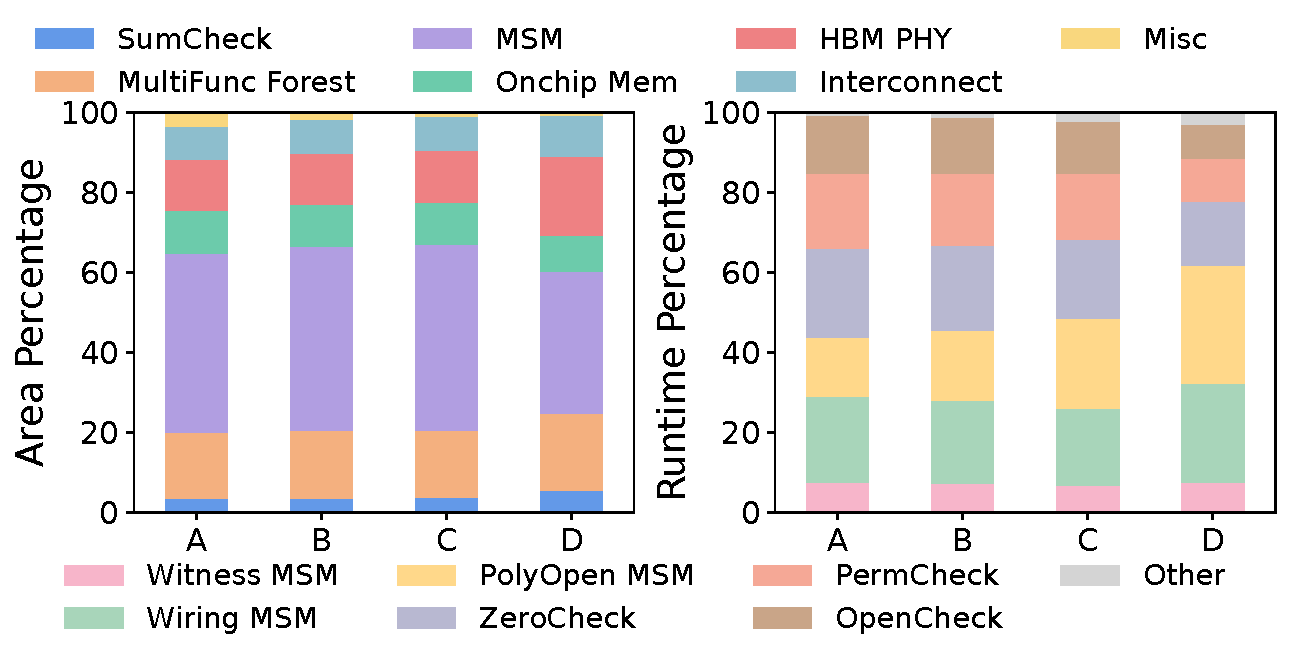
\includegraphics[width=\columnwidth]{area_breakdown_pareto_points_hpca_new.pdf}
    \caption{Area (left, top legend) and runtime (right, bottom legend) breakdowns for the selected Pareto points in \autoref{fig:pareto_plot}.}
    \label{fig:area_breakdown}
\end{figure}

\begin{figure}[t!]
    \centering
    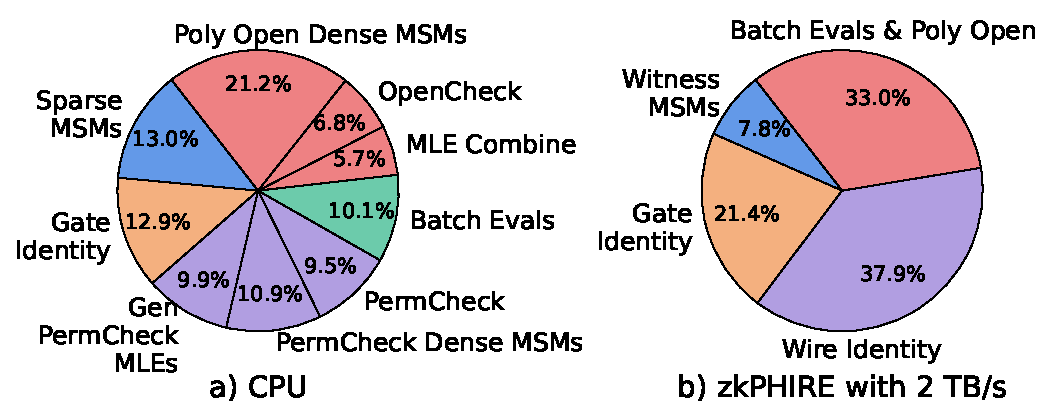
\includegraphics[width=\linewidth]{combined_runtime_breakdown.pdf}
    \caption{Runtime breakdown for CPU and zkPHIRE for $2^{24}$ Jellyfish gates. CPU's sequential execution enables finer breakdowns compared to zkPHIRE.}
    \label{fig:runtime_breakdown}
\end{figure}

\subsubsection{Area, Runtime, and Power}

In \autoref{fig:area_breakdown}, we analyze selected Pareto points from \autoref{fig:pareto_plot}. Across all points, MSM dominates the area as expected.
As the bandwidth increases, both MultiFunction Forest and MSM portions increase, but from C to D, the absolute MSM area remains unchanged while the SumCheck and Forest area increase.
This is also evident in the runtime breakdown: from C to D, the SumCheck portions (ZeroCheck, PermCheck, and OpenCheck) become smaller. Because SumCheck is memory-bound, higher bandwidth incentivizes more resource allocation towards SumCheck-related compute. For low-performance designs, less bandwidth is required, so the MSM is allocated a higher area portion. 


\begin{table}
\caption{Area and power of zkPHIRE. Other includes the Permutation Quotient Generator, MLE Combine and SHA3 units.
}
\label{tab:all_area_power}
\footnotesize
\resizebox{0.98\columnwidth}{!}{
\setlength{\tabcolsep}{1mm}{
\begin{tabular}{lrr}
\hline
& \multicolumn{1}{l}{\textbf{Area (mm²)}} & \multicolumn{1}{l}{\textbf{Average Power (W)}} \\ \hline
MSM (32 PEs)                 & 105.69                                  & 58.99                                          \\
Multifunc Forest ({80} Trees)  & 48.18                                   & {40.69}                                          \\
SumCheck (16 PEs)            & 16.65                                   & 14.43                                          \\
Other                        & {10.64}                                    & {6.17}                                           \\ \hline
\textbf{Total Compute}       & \textbf{181.15}                         & {\textbf{120.29}}                                \\ \hline
SRAM                         & {27.55} & {3.56}                                \\
Interconnect                 & 26.42                                   & 14.83                                          \\
HBM3 (2 PHYs)                & 59.20                                   & 63.60                                          \\
\textbf{Total Memory System} & \textbf{{113.18}}                         & \textbf{{81.99}}                                 \\ \hline
\textbf{Total}               & \textbf{294.32}                         & \textbf{{202.28}}                                \\ \hline
\end{tabular}
}
}
\end{table}

Table~\ref{tab:all_area_power} shows an exemplar zkPHIRE design point we choose for the following analysis. 
In this 294 mm$^2$ design, there are 32 MSM PEs, with {8} modular multipliers per Multifunction tree PE, and 7 EEs and 5 PLs per SumCheck PE. 
The design runs on 2 TB/s HBM bandwidth. 
We use two 32$\times$32 bit-sliced crossbars~\cite{samardzic2021_F1, kim2022_BTS, passas2012crossbar} in the MSM and SumCheck unit, with a shared-bus to form the on-chip bandwidth (up to 19 TB/s) between modules. 
Figure~\ref{fig:runtime_breakdown} further breaks down the runtime to compare with HyperPlonk on CPU.
The colors indicate the same HyperPlonk step between CPU and zkPHIRE running at the configuration of \autoref{tab:all_area_power}. 
We show the latency breakdown for Gate and Wire Identities before performing ZeroCheck masking to show their initial runtime proportions. MSMs dominate runtime before and after  acceleration, though compared to zkSpeed's CPU baseline~\cite{zkspeed2025}, SumChecks take more runtime because the polynomials are complex, exerting more memory pressure on the CPU.


\subsubsection{The On-Chip Memory Trade-off} Since our design space exploration (DSE) sweeps per-MLE capacity (1K - 16K words), we can assess the performance impacts of data reuse via larger scratchpads. 
Our DSE found that performance–area Pareto-optimal designs consistently select SumCheck units with less SRAM in favor of higher compute parallelism (e.g., more PEs/EEs/PLs).
For example, from Figure 10, the Pareto front contains a 100 mm$^2$ design (376 ms runtime) with 8 MSM PEs, 4 SumCheck PEs (4 EEs, 7 PLs), and 4K sized SRAMs. 
Increasing PLs from 7 to 8, we get a 104 mm$^2$ design and 366 ms, which is still Pareto optimal.
If we instead increase the SRAM size to 16K, we get a 108 mm$^2$ design at 368 ms. 
While this improves performance, it is not Pareto optimal. 
Therefore, increasing scratchpad size does improve performance but may not offer the best performance per area.



\begin{figure}[t!]
    \centering
    
    \hspace*{-.7cm}
    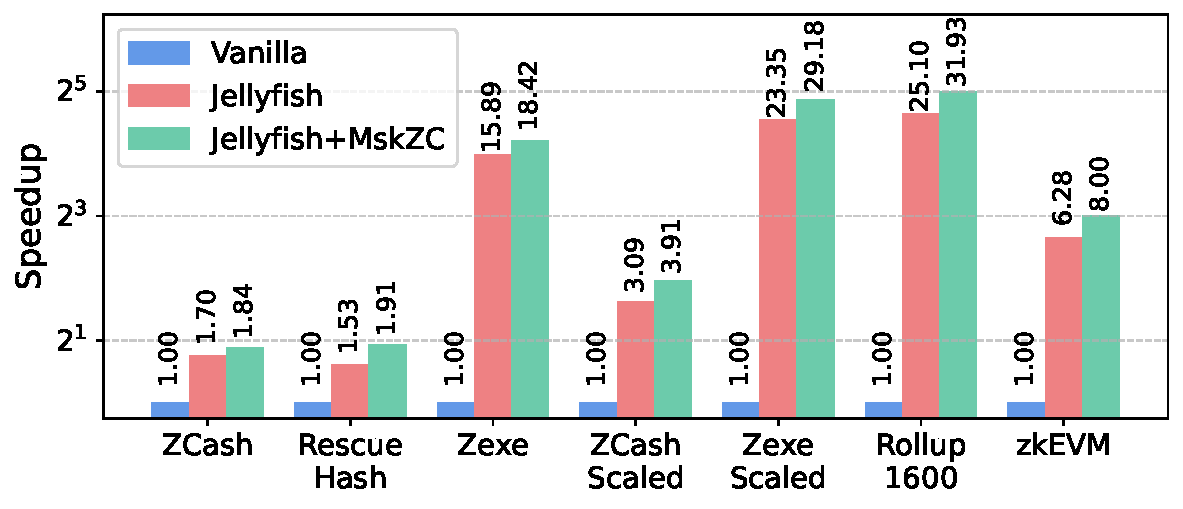
\includegraphics[width=\columnwidth]{optimization_tests.pdf}
    \caption{zkPHIRE speedups across workloads relative to Vanilla Gates. MskZC = Masked ZeroCheck optimization.}
    \label{fig:optimization_tests}
\end{figure}

\begin{figure}[t!]
    \centering    
    \hspace*{-.75cm}
    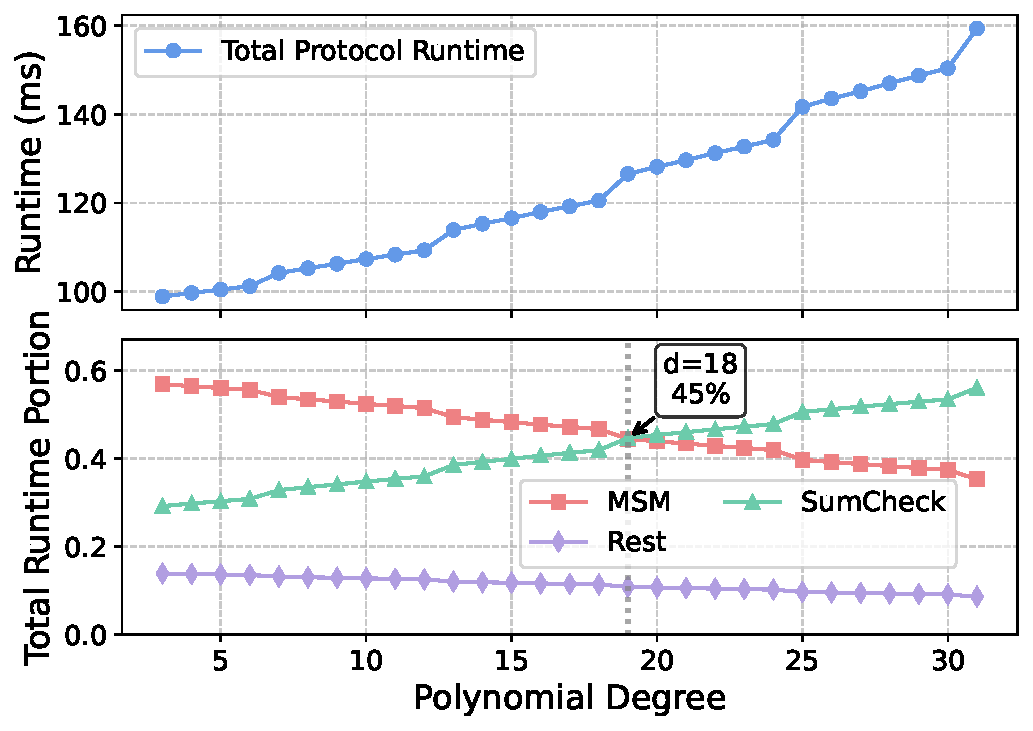
\includegraphics[width=\columnwidth]{runtime_vs_degree_multiple_vars.pdf}
    \caption{High-degree sweep on overall HyperPlonk Protocol. Crossover point is noted. $f = q_1w_1 + q_2w_2 + q_3w_1^{d-1}w_2 + qc$.}
    \label{fig:crossover}
\end{figure}

\subsubsection{Performance from Protocol-level Optimizations}
\autoref{fig:optimization_tests} quantifies the benefits of using Jellyfish gates and masking ZeroCheck latency across several workloads, since different workloads may respond differently to Jellyfish-style mappings. For large workloads, where the Jellyfish gate count is $> 2^{20}$, the speedups from Jellyfish alone reasonably reach what we expect from table size reduction alone. For smaller workloads, we see lower speedups from Jellyfish alone due to serialization overheads of MSMs and other off-chip memory overheads (e.g. fill/drain latencies) that are dwarfed for large workloads. To highlight this, we test scaled up versions of Zcash and Zexe to $2^{24}$ and $2^{25}$ (as done previously \cite{nocap}), and observe $3.1\times$ and $23.3\times$ speedups from Jellyfish alone. For zkEVM, no estimation of Vanilla gates is available \cite{hyperplonk}; we estimate an $8\times$ reduction to highlight our speedup trends for a hypothetical case. ZeroCheck masking provides additional gains of roughly 25-27\% for most workloads, which is what we expect from Amdahl's law by inspecting \autoref{fig:runtime_breakdown}. 

\subsubsection{High-Degree Sweep}
In \autoref{fig:crossover}, we plot the runtime of the highlighted design point over custom gates represented by $f = q_1w_1 + q_2w_2 + q_3w_1^{d-1}w_2 + qc$. For this family of gates, the number of witnesses is fixed, so the total MSM runtime is constant across all values of $d$. Consequently, there is a crossover point after which SumChecks dominate the total protocol runtime. This highlights a key design trade-off: while higher-degree gates reduce overall gate count, they can potentially shift the performance bottleneck from MSMs to SumChecks. Protocol designers must therefore balance gate expressivity with the rising cost of polynomial verification.


\begin{table}[]
\caption{Runtime Comparison with zkSpeed+ and CPU for Vanilla gates (speedups are relative to CPU).}
\label{tab:iso_zkspeed_comp}
\resizebox{\columnwidth}{!}{%
\begin{tabular}{|c|c|ccc|}
\hline
\multirow{2}{*}{Workload} & \multirow{2}{*}{Gates} & \multicolumn{3}{c|}{Runtime (ms)} \\ \cline{3-5} 
 &  & \multicolumn{1}{c|}{CPU} & \multicolumn{1}{c|}{zkSpeed+} & zkPHIRE \\ \hline
ZCash & 2\textsuperscript{17} & \multicolumn{1}{c|}{1429} & \multicolumn{1}{c|}{1.825 (783$\times$)} & 2.012 (710$\times$) \\ \hline
Auction & 2\textsuperscript{20} & \multicolumn{1}{c|}{8619} & \multicolumn{1}{c|}{10.171 (847$\times$)} & 10.88 (792$\times$) \\ \hline
2\textsuperscript{12} Rescue Hashes & 2\textsuperscript{21} & \multicolumn{1}{c|}{18637} & \multicolumn{1}{c|}{19.631 (888$\times$)} & 20.977 (1822$\times$) \\ \hline
Zexe's Recursive Ckt & 2\textsuperscript{22} & \multicolumn{1}{c|}{37469} & \multicolumn{1}{c|}{38.535 (972$\times$)} & 41.117 (911$\times$) \\ \hline
Rollup of 10 Pvt Tx & 2\textsuperscript{23} & \multicolumn{1}{c|}{74052} & \multicolumn{1}{c|}{76.356 (969$\times$)} & 81.362 (910$\times$) \\ \hline
Rollup of 25 Pvt Tx & 2\textsuperscript{24} & \multicolumn{1}{c|}{145500} & \multicolumn{1}{c|}{151.973 (957$\times$)} & 161.876 (898$\times$) \\ \hline
Rollup of 50 Pvt Tx & 2\textsuperscript{25} & \multicolumn{1}{c|}{325048} & \multicolumn{1}{c|}{---} & 322.922 (1006$\times$) \\ \hline
Rollup of 100 Pvt Tx & 2\textsuperscript{26} & \multicolumn{1}{c|}{640987} & \multicolumn{1}{c|}{---} & 645.029 (994$\times$) \\ \hline
\end{tabular}%
}
\end{table}

\subsubsection{Performance Comparison}
\label{sec:perf_comp}
\autoref{tab:iso_zkspeed_comp} compares a 300 mm$^2$ zkPHIRE design using the same modular multipliers as zkSpeed+ (366 mm$^2$ with MLE Updates pipelined into SumCheck) and without ZeroCheck masking. This is to provide as fair a comparison as possible (zkSpeed+ is roughly $10\%$ faster than zkSpeed). Speedups are reported relative to CPU. zkPHIRE is about $10\%$ slower than zkSpeed+, while offering flexibility to support arbitrary, custom gates. \autoref{tab:iso_cpu_comp} shows zkPHIRE's speedups at iso-CPU area (294 mm$^2$) with fixed primes and ZeroCheck masking, achieving $1486\times$ geomean speedup and generating proofs for workloads upwards of $2^{30}$ nominal gates. Lastly,  \autoref{tab:iso_app_comp} compares the same design (with ZeroCheck masking and fixed primes) with zkSpeed+ at iso-application, achieving geomean $11.87\times$ speedup.




\begin{table}[]
\caption{Runtime and speedup compared to CPU for Jellyfish gates. Vanilla gate counts are shown to show original problem size. }
\label{tab:iso_cpu_comp}
\resizebox{\columnwidth}{!}{%
\begin{tabular}{|c|cc|cc|}
\hline
\multirow{2}{*}{Workload} & \multicolumn{2}{c|}{Gates} & \multicolumn{2}{c|}{Runtime (ms)} \\ \cline{2-5} 
 & \multicolumn{1}{c|}{Vanilla} & Jellyfish & \multicolumn{1}{c|}{CPU} & zkPHIRE \\ \hline
ZCash & \multicolumn{1}{c|}{2\textsuperscript{17}} & 2\textsuperscript{15} & \multicolumn{1}{c|}{701} & 0.750 (934$\times$) \\ \hline
Zexe Recursive Ckt & \multicolumn{1}{c|}{2\textsuperscript{22}} & 2\textsuperscript{17} & \multicolumn{1}{c|}{1951} & 1.440 (1354$\times$) \\ \hline
Rollup of 10 Pvt Tx & \multicolumn{1}{c|}{2\textsuperscript{23}} & 2\textsuperscript{18} & \multicolumn{1}{c|}{3339} & 2.269 (1471$\times$) \\ \hline
Rollup of 25 Pvt Tx & \multicolumn{1}{c|}{2\textsuperscript{24}} & 2\textsuperscript{19} & \multicolumn{1}{c|}{6161} & 3.874 (1590$\times$) \\ \hline
2\textsuperscript{12} Rescue Hashes & \multicolumn{1}{c|}{2\textsuperscript{21}} & 2\textsuperscript{20} & \multicolumn{1}{c|}{11532} & 7.114 (1621$\times$) \\ \hline
Rollup of 50 Pvt Tx & \multicolumn{1}{c|}{2\textsuperscript{25}} & 2\textsuperscript{20} & \multicolumn{1}{c|}{11533} & 7.114 (1621$\times$) \\ \hline
Rollup of 100 Pvt Tx & \multicolumn{1}{c|}{2\textsuperscript{26}} & 2\textsuperscript{21} & \multicolumn{1}{c|}{24071} & 13.614 (1474$\times$) \\ \hline
Rollup of 1600 Pvt Tx & \multicolumn{1}{c|}{2\textsuperscript{30}} & 2\textsuperscript{25} & \multicolumn{1}{c|}{355406} & 207.673 (1711$\times$) \\ \hline
zkEVM & \multicolumn{1}{c|}{---} & 2\textsuperscript{27} & \multicolumn{1}{c|}{25 min} & 828.948 (1809$\times$) \\ \hline
\end{tabular}%
}
\end{table}

\begin{table}[]
\caption{Iso-application comparison of zkSpeed+ (Vanilla)\\and zkPHIRE (Jellyfish).}
\label{tab:iso_app_comp}
\resizebox{\columnwidth}{!}{%
\begin{tabular}{|c|cc|cc|}
\hline
\multirow{2}{*}{Workload} & \multicolumn{2}{c|}{Gates} & \multicolumn{2}{c|}{Runtime (ms)} \\ \cline{2-5} 
 & \multicolumn{1}{c|}{Vanilla} & Jellyfish & \multicolumn{1}{c|}{zkSpeed+} & zkPHIRE \\ \hline
ZCash & \multicolumn{1}{c|}{2\textsuperscript{17}} & 2\textsuperscript{15} & \multicolumn{1}{c|}{1.825} & 0.750 (2.43$\times$) \\ \hline
2\textsuperscript{12} Rescue Hashes & \multicolumn{1}{c|}{2\textsuperscript{21}} & 2\textsuperscript{20} & \multicolumn{1}{c|}{19.631} & 7.114 (2.75$\times$) \\ \hline
Zexe Recursive Circuit & \multicolumn{1}{c|}{2\textsuperscript{22}} & 2\textsuperscript{17} & \multicolumn{1}{c|}{38.535} & 1.440 (26.76$\times$) \\ \hline
Rollup of 10 Pvt Tx & \multicolumn{1}{c|}{2\textsuperscript{23}} & 2\textsuperscript{18} & \multicolumn{1}{c|}{76.356} & 2.269 (33.65$\times$) \\ \hline
Rollup of 25 Pvt Tx & \multicolumn{1}{c|}{2\textsuperscript{24}} & 2\textsuperscript{19} & \multicolumn{1}{c|}{151.973} & 3.874 (39.23$\times$) \\ \hline
\end{tabular}
}
\end{table}

